\section{Introduction}

Chapter 2 introduced a Thurstonian choice model and showed that, conditioned on estimated parameters, the model can systematically predict the repulsion effect, but not the attraction effect. This chapter tests another prediction of the model while demonstrating a novel empirical result in another domain: best-worst choice.

\subsection{Introducing Best-Worst Choice}

Best-worst choice is an experimental paradigm where participants select their most and least preferred options from a choice set. Originally proposed by \textcite{finn1992determining}, best-worst choice is widely used in a number of applied fields, such as transportation \parencite{beck2016best} and healthcare economics \parencite{cheung2016using,flynn2007best,muhlbacher2016experimental}. One key advantage, when compared to standard choice research, is that researchers can use best-worst choices to gain information about participants' ranking of options while never requiring them to complete a full ranking task \parencite{flynn2014best}.

Researchers have developed theoretical models to account for best-worst choice data. These models relate best-worst choices to underlying utility functions. \textcite{marleyProbabilisticModelsBest2005} developed a class of models known as the \textit{maxdiff} (maximum difference) model of best-worst choice\footnote{Note that the term maxdiff is sometimes erroneously used to refer to best-worst experiments in the generic sense. Following \textcite{marleyProbabilisticModelsBest2005}, maxdiff refers to a specific class and parameterization of a best-worst choice model.}. According to the maxdiff model, the joint probability of selecting both option $j$ as best and also option $k$ as worst (denoted $BW(j,k|K)$ ) from set $K$, where $j \neq k$, is computed as:

\begin{equation}
   BW(j,k|K)=\frac{e^{u_{j}-u_{k}}}{\sum_{\substack{{p,q}\in K\\p \neq q}} e^{u_{p}-u_{q}}}   
   \label{eqn:maxdiff_equation_joint}
\end{equation}

where $u_{i}$ is the utility of option $i$. This model proposes that a single utility scale determines the selection of both the best option and the worst option in a choice set. It assumes that best choice probabilities are an increasing function of $u$, while worst choice probabilities are a decreasing function of $u$. Furthermore, the maxdiff model relies on the differences of utilities; From a given choice set, the most likely best-worst pair is the pair with the largest difference in utility values. Utilities are also assumed to be independent of each other. Note that the use of the exponential function means that the maxdiff model is another form of the widely used multinomial logit (MNL) choice model \parencite{hausman1984specification}. 

There are several variants of the maxdiff model along with other best-worst choice models \parencite{marleyProbabilisticModelsBest2005,marleyProbabilisticModelsSetdependent2008,marleyModelsBestWorst2012,flynnBestWorstScaling2007,flynn2014best}, though the maxdiff model from Equation~\ref{eqn:maxdiff_equation_joint} remains the dominant model for analyzing best-worst choice data \parencite{hawkinsBestTimesWorst2014}.

The marginal probability $B(j|K)$ of selecting option $j$ as best from set $K$ can be written as:

\begin{equation}
   B(j|K)=\frac{e^{u_{j}}}{\sum_{\substack{{p}\in K}} e^{u_{p}}}
\end{equation}

while the marginal probability $W(k|K)$ of selecting option $k$ as worst from set $K$ can be written as:

\begin{equation}
   W(j|K)=\frac{e^{-u_{j}}}{\sum_{\substack{{p}\in K}} e^{-u_{p}}}
\end{equation}

Best-choice probabilities are an increasing function of $u$, while worst choice probabilities are a decreasing function of $u$.

The maxdiff model predicts a decreasing monotonic relationship between best choice probabilities and worst choice probabilities \parencite{hawkinsBestTimesWorst2014}. Options most likely to be chosen as best are necessarily least likely to be chosen as worst, and vice versa. That is, if we assume all options' utilities are independent, the model predicts that best choice probabilities are negatively, monotonically related to worst choice probabilities. 

To demonstrate this, consider the following simulation. $500$ ternary (three-option) best-worst choice trials were simulated, by sampling 3 utilities from the standard normal distribution. For each trial, the marginal best and worst choice probabilities were computed using the maxdiff model. These probabilities were then plotted against each other in a state-trace plot (see Figure~\ref{fig:maxdiff_sim}) \parencite{bamber1979state}. In a state-trace plot, the analyst plots two dependent variables against one another in each experimental condition. 

\begin{figure}
   \centering
   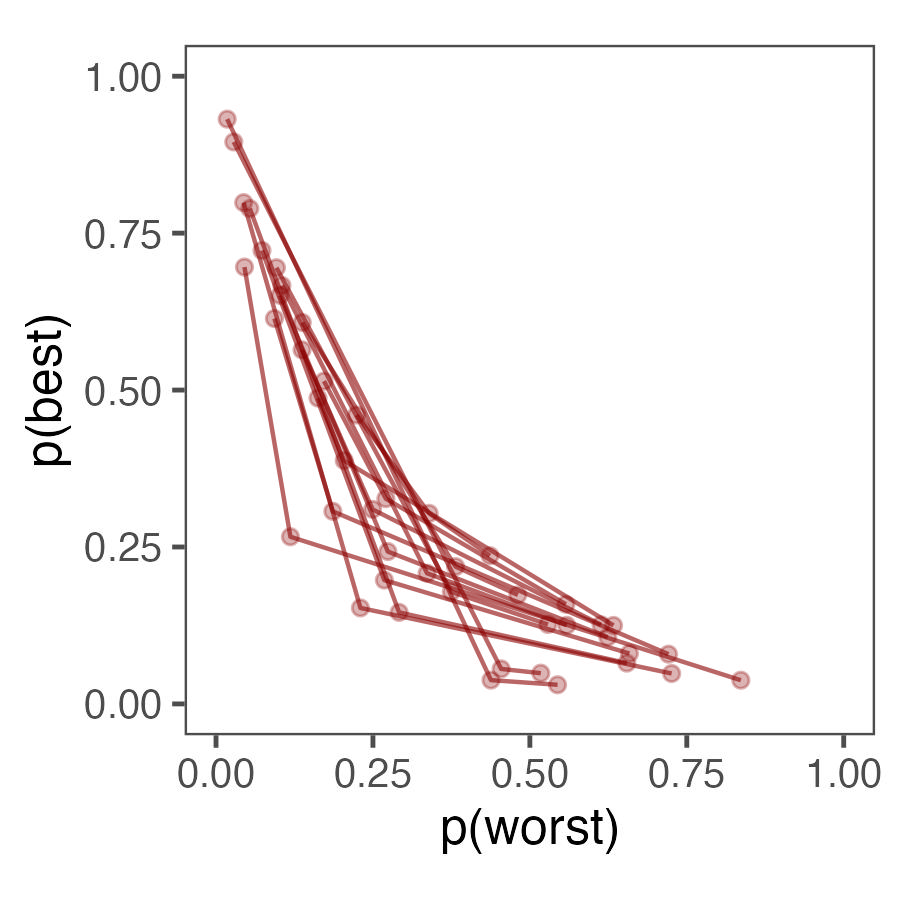
\includegraphics[width=150mm]{figures/maxdiff_sim_monotonic.jpeg}
   \caption{Best-worst choice simulations using the maxdiff model. Each curve is a separate simulation. The model predicts a negative, monotonic relationship between the marginal best choice and worst choice probabilities.}
   \label{fig:maxdiff_sim}
\end{figure}

Researchers have explored whether this monotonicity holds empirically. \textcite{hawkinsIntegratingCognitiveProcess2014a} tested both preferential and perceptual best-worst choice data using response time modeling. They used the Linear Ballistic Accumulator model (LBA) \parencite{brownSimplestCompleteModel2008b}, which casts the decision process as a race between evidence accumulators towards a threshold, where the average accumulation across trials is captured by the drift rate parameter. Modeling both preferential and perceptual best-worst choice data, they were able to successfully account for choice data by assuming a parallel race between best and worst accumulators for each option. Furthermore, they showed that the utility values estimated for each option using an MNL model were positively linearly related to the log drift rate values from the LBA, suggesting an underlying utility representation that explains both best and worst choices. 

In a follow-up article, \textcite{hawkinsBestTimesWorst2014} found that, collapsing across choice sets, best choice probabilities are monotonically related to worst choice probabilities. Options that were most likely to be selected as best were least likely to be selected as worst, and vice versa. This finding held for perceptual choice and consumer choice. They also showed that, using the parallel best-worst LBA, the drift rate parameter for worst choice can be parameterized as the reciprocal of the best choice drift rate. Formally, if $d_{b}(i)$ is the drift rate for selecting option $i$ as best, then $d_{w}(i)=1/d_{b}(i)$, where $d_{w}(i)$ is option $i$'s drift rate for worst choices. 

Implementations of both the parallel best-worst LBA and the maxdiff model assume that the utilities of all options presented are independent. However, as shown below, the Thurstonian choice model from Chapters 1 and 2 predicts, under certain conditions, a dissociation between best and worst choices inconsistent with this assumption.

\subsection{Model-Based Dissociations in Best-Worst Choice}

Below, the Thurstonian choice model from Chapter 2 is used to make a prediction regarding a dissociation between best choices and worst choices. 

Let $K$ be a choice set consisting of options $T$, $C$, and $D$ (i.e., target, competitor, and decoy). As in Experiments 1 and 2, the options are rectangles in a perceptual choice experiment. As in Chapter 2, it is assumed that on each trial $i$ with choice set $K$, the vector $\bm{X_{i}}$ of perceived areas is sampled from a multivariate Gaussian distribution with a mean vector $\boldsymbol{\mu}$ and variance-covariance matrix $\boldsymbol{\Sigma}$:

\begin{equation}
   \bm{X}_{ij} \sim \bm{N}(\boldsymbol{\mu},\boldsymbol{\Sigma})
   \label{eqn:bw_thurstone_dist}
\end{equation}

Given a vector $\bm{X_{i}}$ of perceived areas on trial $i$ with set $K$, according to model, the probability a participant selects stimulus $j$ as best and option $k$ as worst is:

\begin{equation}
   BW_{K}(j,k)=P(\bm{X}_{ij}-\bm{X}_{ik} > \bm{X}_{ip}-\bm{X}_{iq}), \forall p, q \in K, p \neq q
   \label{eqn:bw_thurstone_equation}
\end{equation}

Simply put, on any given trial, the option with the largest perceived area is always selected as best, while the option with the smallest perceived area is always selected as worst. 

Applied to best-worst choice the Thurstonian choice model is somewhat similar to the maxdiff model. There are two main differences between these models, however. First, the Thurstonian model is a version of the Multinomial Probit (MNP) model, while the maxdiff model is a variant of the MNL model. Crucially, however, the Thurstonian model provides a distribution for option utilities and allows for correlations between these utilities, while the maxdiff model generally assumes that these utilities are independent of one another. Note that the latter is a convenience assumption and can of course be relaxed.

However, given the correlations estimated from Experiment 2 , the Thurstonian predicts that, in the best-worst choice paradigm, there is a non-monotonic relationship between marginal best choices and worst choices. This dissociation is explained below.

The Thurstonian choice model, conditioned on the parameters $\boldsymbol{\mu}$ and $\boldsymbol{\Sigma}$ estimated from Experiment 2 was simulated for $1,000,000$ best-worst choice trials\footnote{Only the parameters estimated from the triangle condition (See Experiment 2) were used here, as the parameters estimated from the horizontal condition made identical predictions.}. As in Chapter 2, results are collapsed over choice set (i.e., whether the target is wide or tall). Marginal choice proportions for the target, competitor, and decoy options were computed at each level of TDD. These results are presented in Figure~\ref{fig:bw_sim}, in a series of state-trace plots.

\begin{figure}
   \centering
   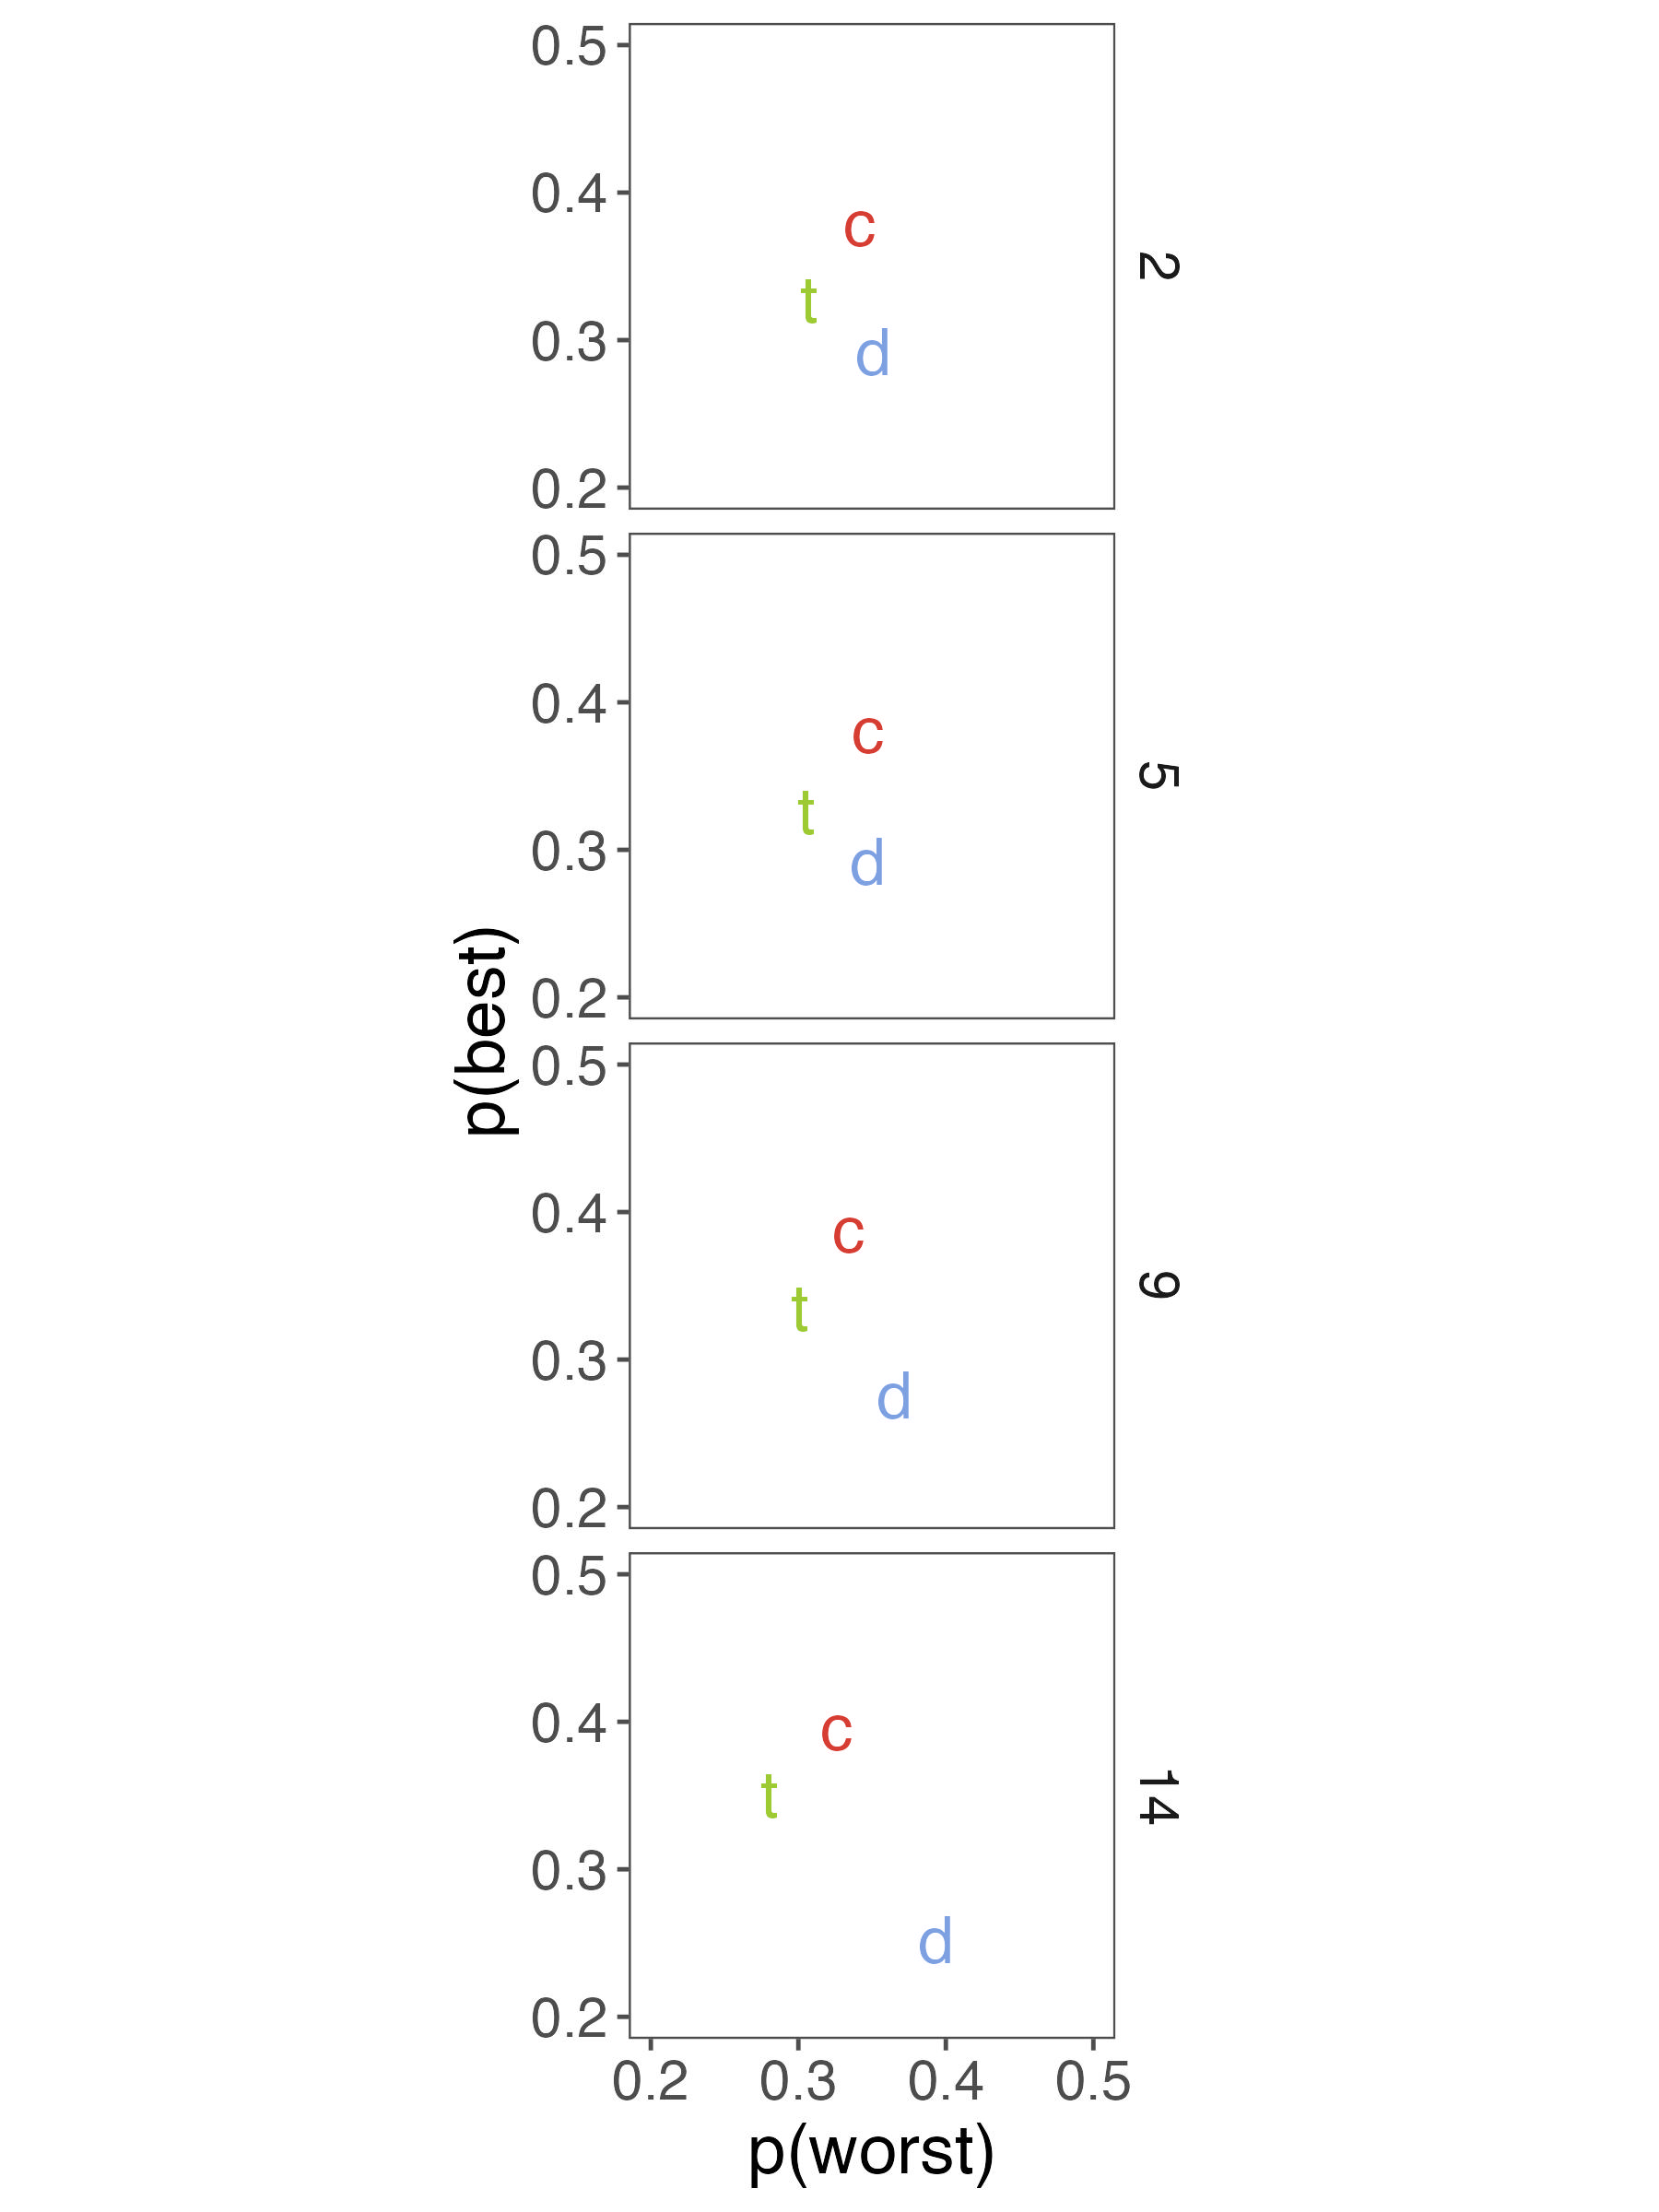
\includegraphics[width=\linewidth]{figures/bw_preds_sigma_constant_comp_effect_no_outliers.jpeg}
   \caption{Simulated best-worst predictions per the Thurstonian choice model. Each row is a different level of TDD.}
   \label{fig:bw_sim}
\end{figure}

The model, conditioned on the estimated parameters, predicts a theoretically informative data pattern. Although the competitor is most frequently chosen as best (as in the empirical results from Experiment 2), it is not least frequently chosen as worst. Specifically, the Thurstonian model predicts that $B(C)>B(T)$ and $W(C)>W(C)$. At lower levels of TDD, the model even predicts that competitor and decoy are chosen as best at similar rates, a prediction likely due to the fact that participants are generally less sensitive to perceptual differences when providing ratings than when making choices \parencite{gronau2023choice}.

The Thurstonian choice model predicts this pattern because $\rho_{TD}>\rho_{CD}\approx\rho_{TC}$. On the relatively few trials where $X_{iD}$ is largest, it is more likely that $X_{iD}>X_{iT}>X_{iC}$ than $X_{iD}>X_{iC}>X_{iT}$. In other words, the high $\rho_{TD}$ value pulls up the target more than the competitor. Though the similarity, and comparability, of target and decoy thus entail that the competitor is chosen more as best compared to the target (as in Experiment 2), this does not necessarily entail that the competitor is chosen less than the target as worst.

This effect is subtle, and the predicted effect size is small. Indeed, all differences in predicted $W(C)-W(T)$ values were $<.05$. Experiment 3 contains the empirical and modeling results from a best-worst choice experiment designed to test this prediction. The dissociation between best and worst choices does indeed occur empirically. Here the monotonicity assumption required by the independent utilities assumption, typical in applications of the maxdiff model, also fails empirically.

\section{Experiment 3}

The goal of Experiment 3 was to test the predictions of the Thurstonian choice model. Specifically, the perceptual model predicts that both $B(C)>B(T)$ and $W(C)>W(T)$. To test this prediction, the stimuli were identical to those of Experiment 2, including the triangle display. The aforementioned prediction holds empirically and the maxdiff model (with independent utilities) cannot account for these results.

\subsection{Methods}

\subsubsection{Participants.}
Data collection took place at the University of Massachusetts Amherst. $392$ undergraduate students participated in exchange for course credit. $23$ participants who achieved less than $80\%$ accuracy on catch trials (see below) were excluded from all analyses. 

From the remaining $369$ participants, $2,604$ trials with first-choice response times (RTs) $<100\text{ms}$ or $>10000\text{ms}$ were also excluded from all analyses, leaving $107,727$ trials across all participants.

Participants were randomly assigned into one of two conditions: best-worst or worst-best. On each trial, participants in the best-worst condition first chose the largest rectangle and then chose the smallest rectangle. Participants in the worst-best condition chose in the opposite order. The order condition was included to account for the possibility that best-worst choice order impacts choice, though results were qualitatively identical across conditions, so all results are collapsed across order. 

After removing participants, there were $185$ participants in the best-worst condition and $184$ participants in the worst-best condition.

\subsubsection{Stimuli.}
The experiment had three types of trials: critical trials, filler trials, and catch trials. 

Stimuli on critical trials were identical to those of Experiment 2. On each critical trial, the target and competitor had the same area but differed on orientation, with one stimulus being wide and the other tall. The decoy always had the same orientation as the target. TDD varied at $2\%$, $5\%$, $9\%$, and $14\%$. Target, competitor, and decoy rectangles along three diagonals, as in Experiment 2 (see Figure~\ref{fig:e2_stim}). 

On each filler trial, three stimuli were uniformly sampled from the space between the largest and smallest diagonals (see Figure~\ref{fig:e2_stim}).

On each catch trial, one stimulus was sampled from the largest diagonal, while two stimuli were sampled from the smallest diagonal.

\subsubsection{Design.}
There were 8 blocks of trials. In each block there were 24 critical trials, 6 at each TDD level. There were 8 trials per diagonal. In addition to the critical trials, there were 10 filler trials and 3 catch trials per block.

Participants were randomly assigned into one of two conditions: best-worst or worst-best, as described above. 

Stimuli were presented on computer monitors with a resolution of 1920 x 1080 pixels. The experiment was programmed with GNU Octave and Psychtoolbox \parencite{octave,brainardPsychophysicsToolbox1997}. 

\subsubsection{Procedure.}

The experiment began with three practice trials, which were identical to the filler trials. 

On each trial, participants saw three rectangles, labeled 1, 2, and 3 (from left to right), arranged in a triangle display. Participants in the best-worst (worst-best) condition saw a prompt asking them to select the largest (smallest) rectangle on screen. Participants used the mouse to select their choice. After they made their choice, their chosen rectangle changed color to indicate that it was no longer available as an option. Next, participants in the best-worst (worst-best) condition selected the smallest (largest) rectangle, at which point the trial ended. See Figure~\ref{fig:bw_example_trial} for an example trial.

\begin{figure}
   \centering
   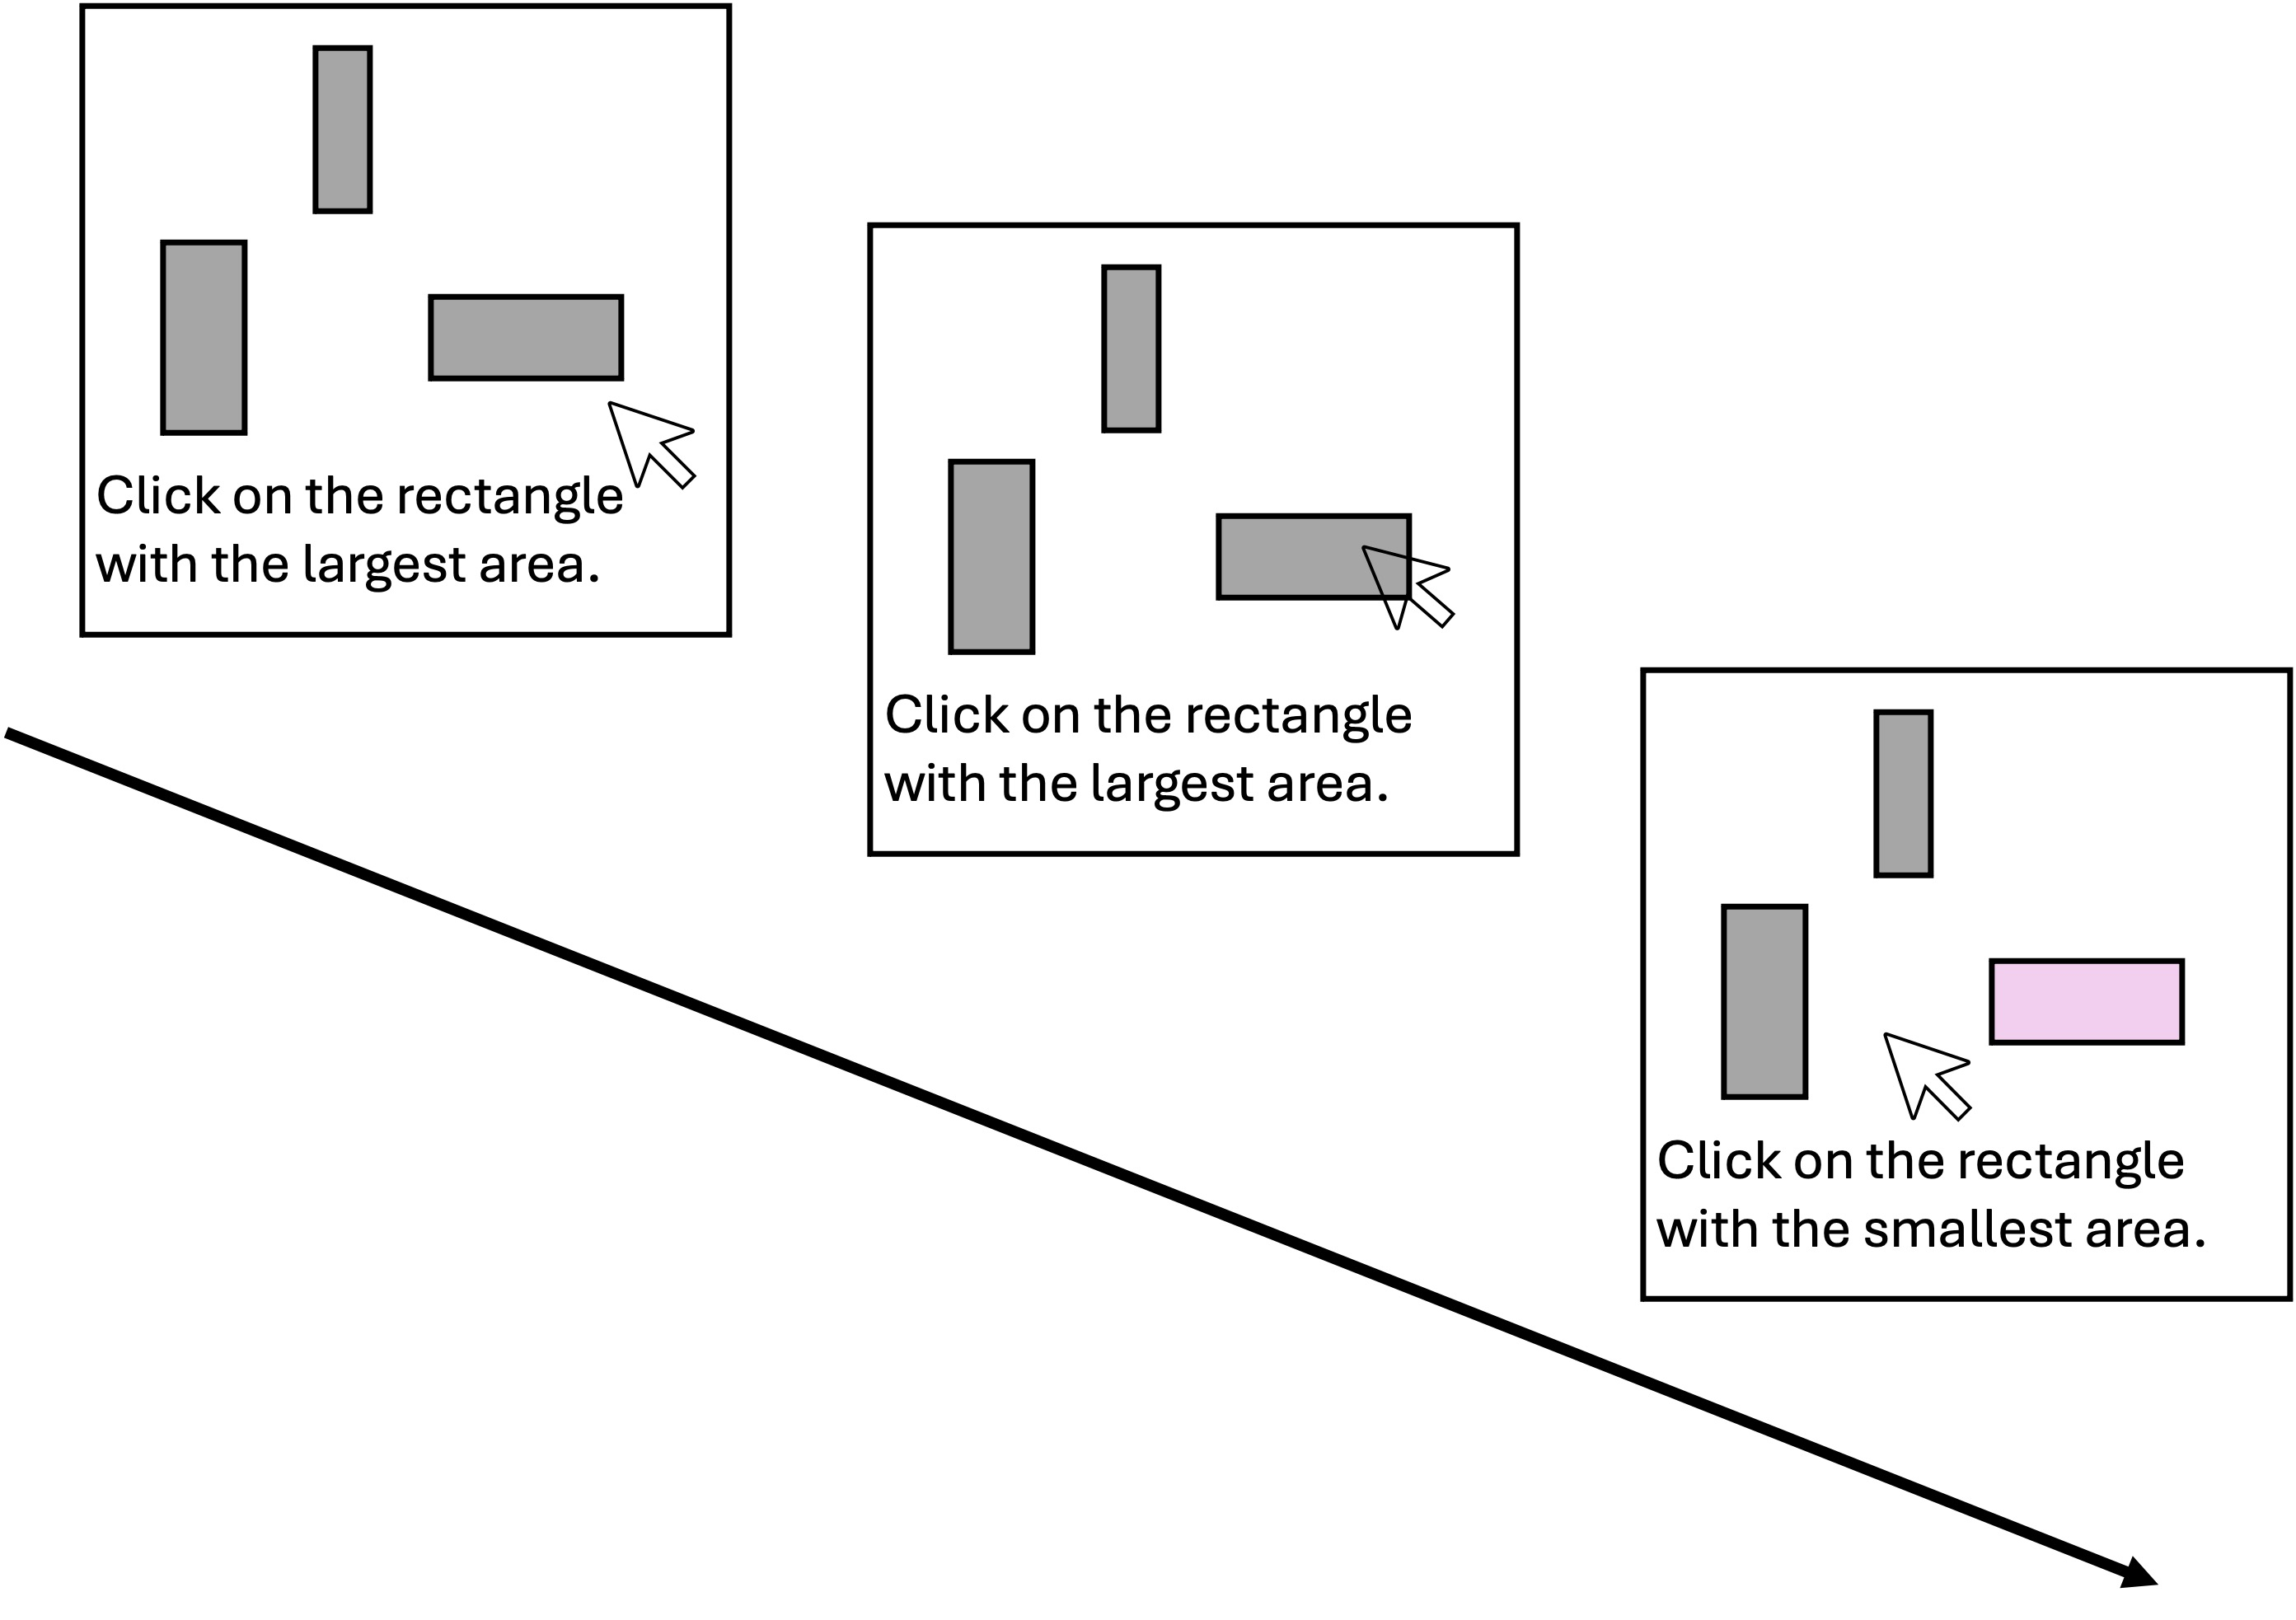
\includegraphics[width=\linewidth]{figures/bw_design_fig.jpg}
   \caption{A sample experimental trial from Experiment 3. This is a trial in the best-worst condition.}
   \label{fig:bw_example_trial}
 \end{figure}
 
Stimulus order was randomized on each trial. 

Participants were told their percentage correct for best choices, worst choices, and overall choices at the end of the experiment.

\subsection{Results}

\subsubsection{Catch Trials.}
Participants performed well on the catch trials. The mean percentage correct for best choices was $97.97\% (SD=14.09)$, and the mean percentage correct for worst choices was $98.26\% (SD=13.09)$. The mean percentage correct for both best and worst choices (i.e., the mean percentage of the trials on which participants were able to correctly identify the largest and smallest rectangles) was $96.98\% (SD=17.12)$. 

\subsubsection{Filler Trials.}
Participants performed worse on the filler trials compared to the catch trials, but still well above chance. The mean percentage correct for best choices was $89.83\% (SD=30.23)$, and the mean percentage correct for worst choices was $88.95\% (SD=41.35)$. The mean percentage correct for both best and worst choices was $80.95\% (SD=39.37)$. 

\subsubsection{Critical Trials.}

% First, I computed the mean choice proportions for each distinct rectangle, collapsed across choice set. Here, I replicated the findings of \textcite{hawkinsBestTimesWorst2014}, that, when ignoring the effect of context, best choices and worst choices are monotonically related. These data are plotted in Figure~\ref{fig:bw_marginal}.

% \begin{figure}
%    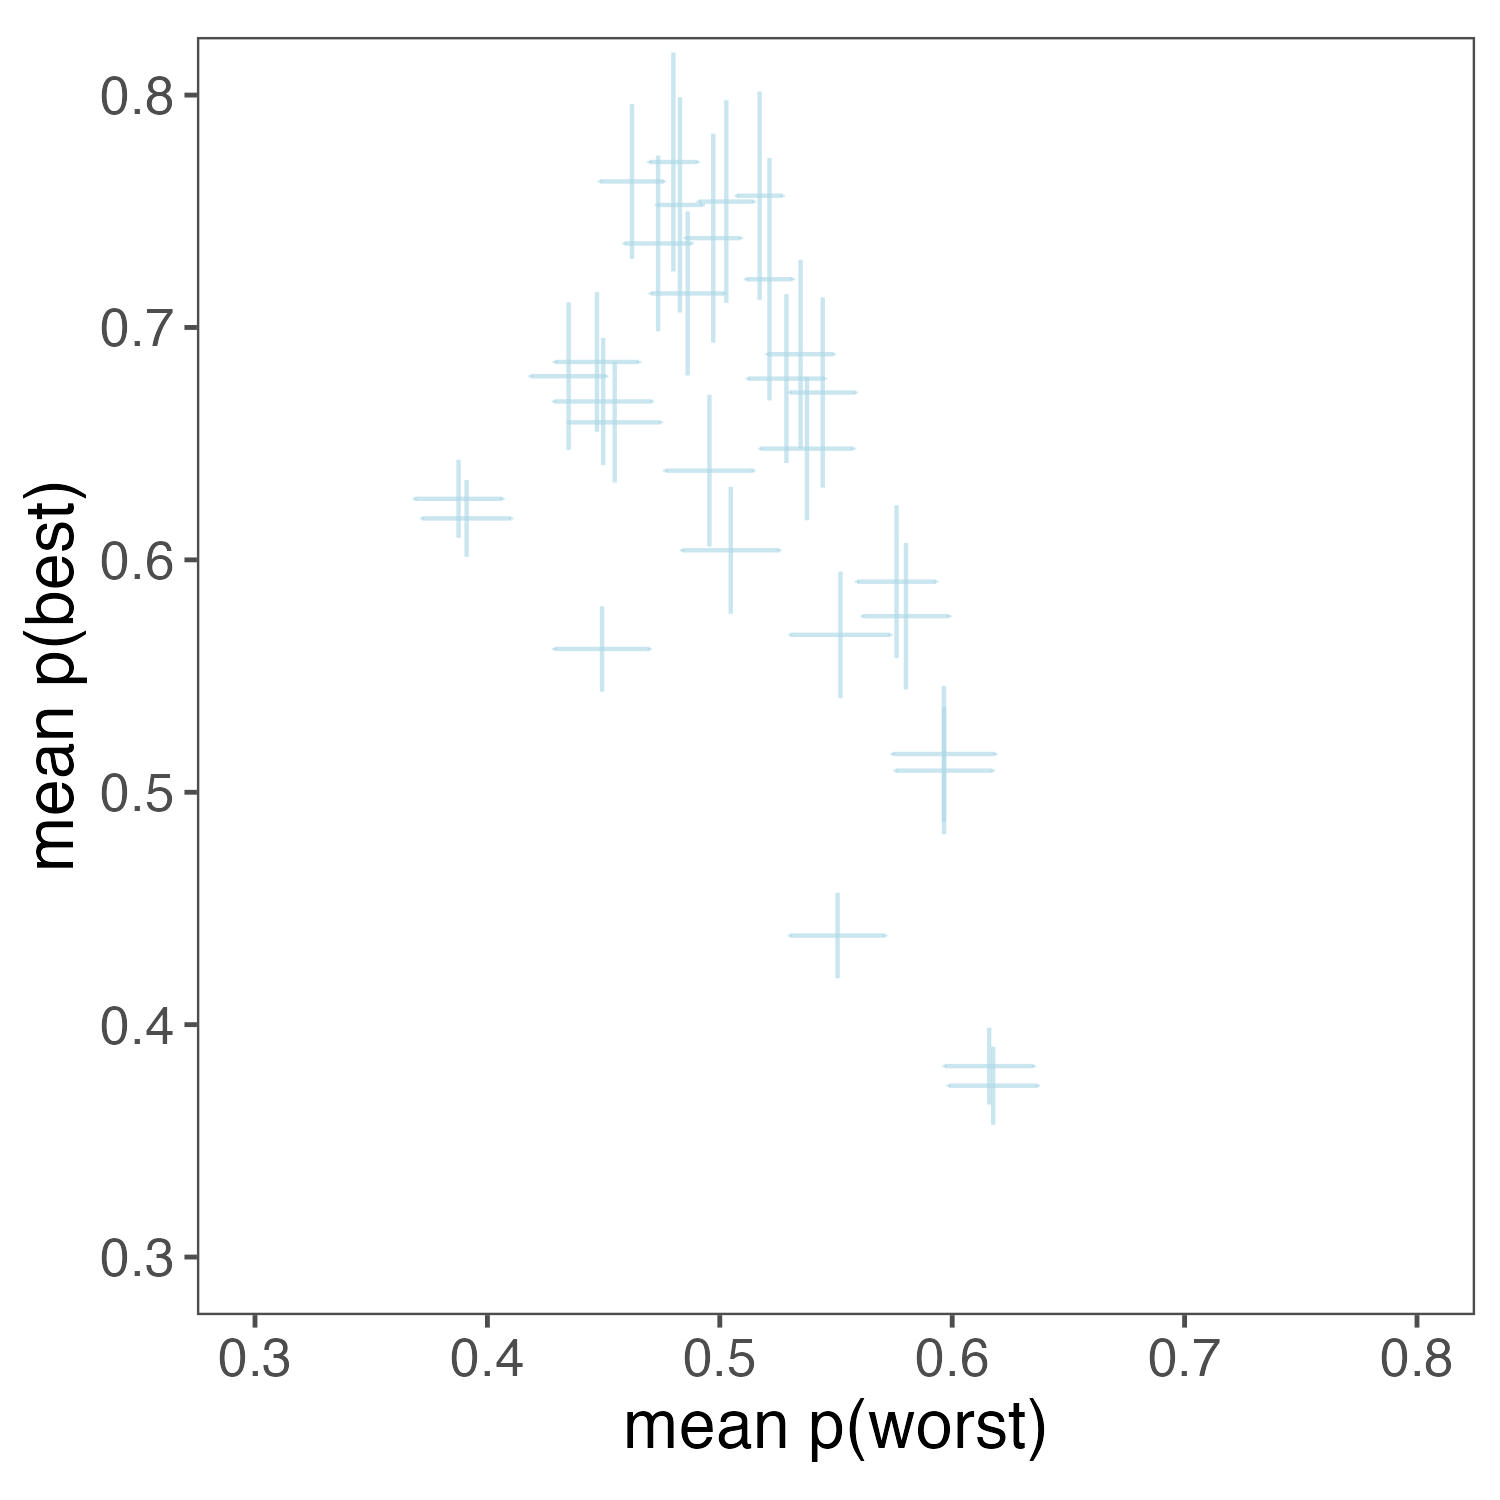
\includegraphics[width=\linewidth]{figures/crit_mean_props_marginal.jpeg}
%    \caption{Experiment 3 marginal mean best and worst choice proportions for all unique rectangles, collapsed across choice set. X and Y axis error bars are $95\%$ CIs.}
%    \label{fig:bw_marginal}
% \end{figure}

First, data were analyzed by computing choice proportions for each option conditioned on TDD and choice set. Mean choice proportions for these data are plotted in Figure~\ref{fig:bw_mean_choice} (left and middle columns). 

\begin{figure}
   \centering
   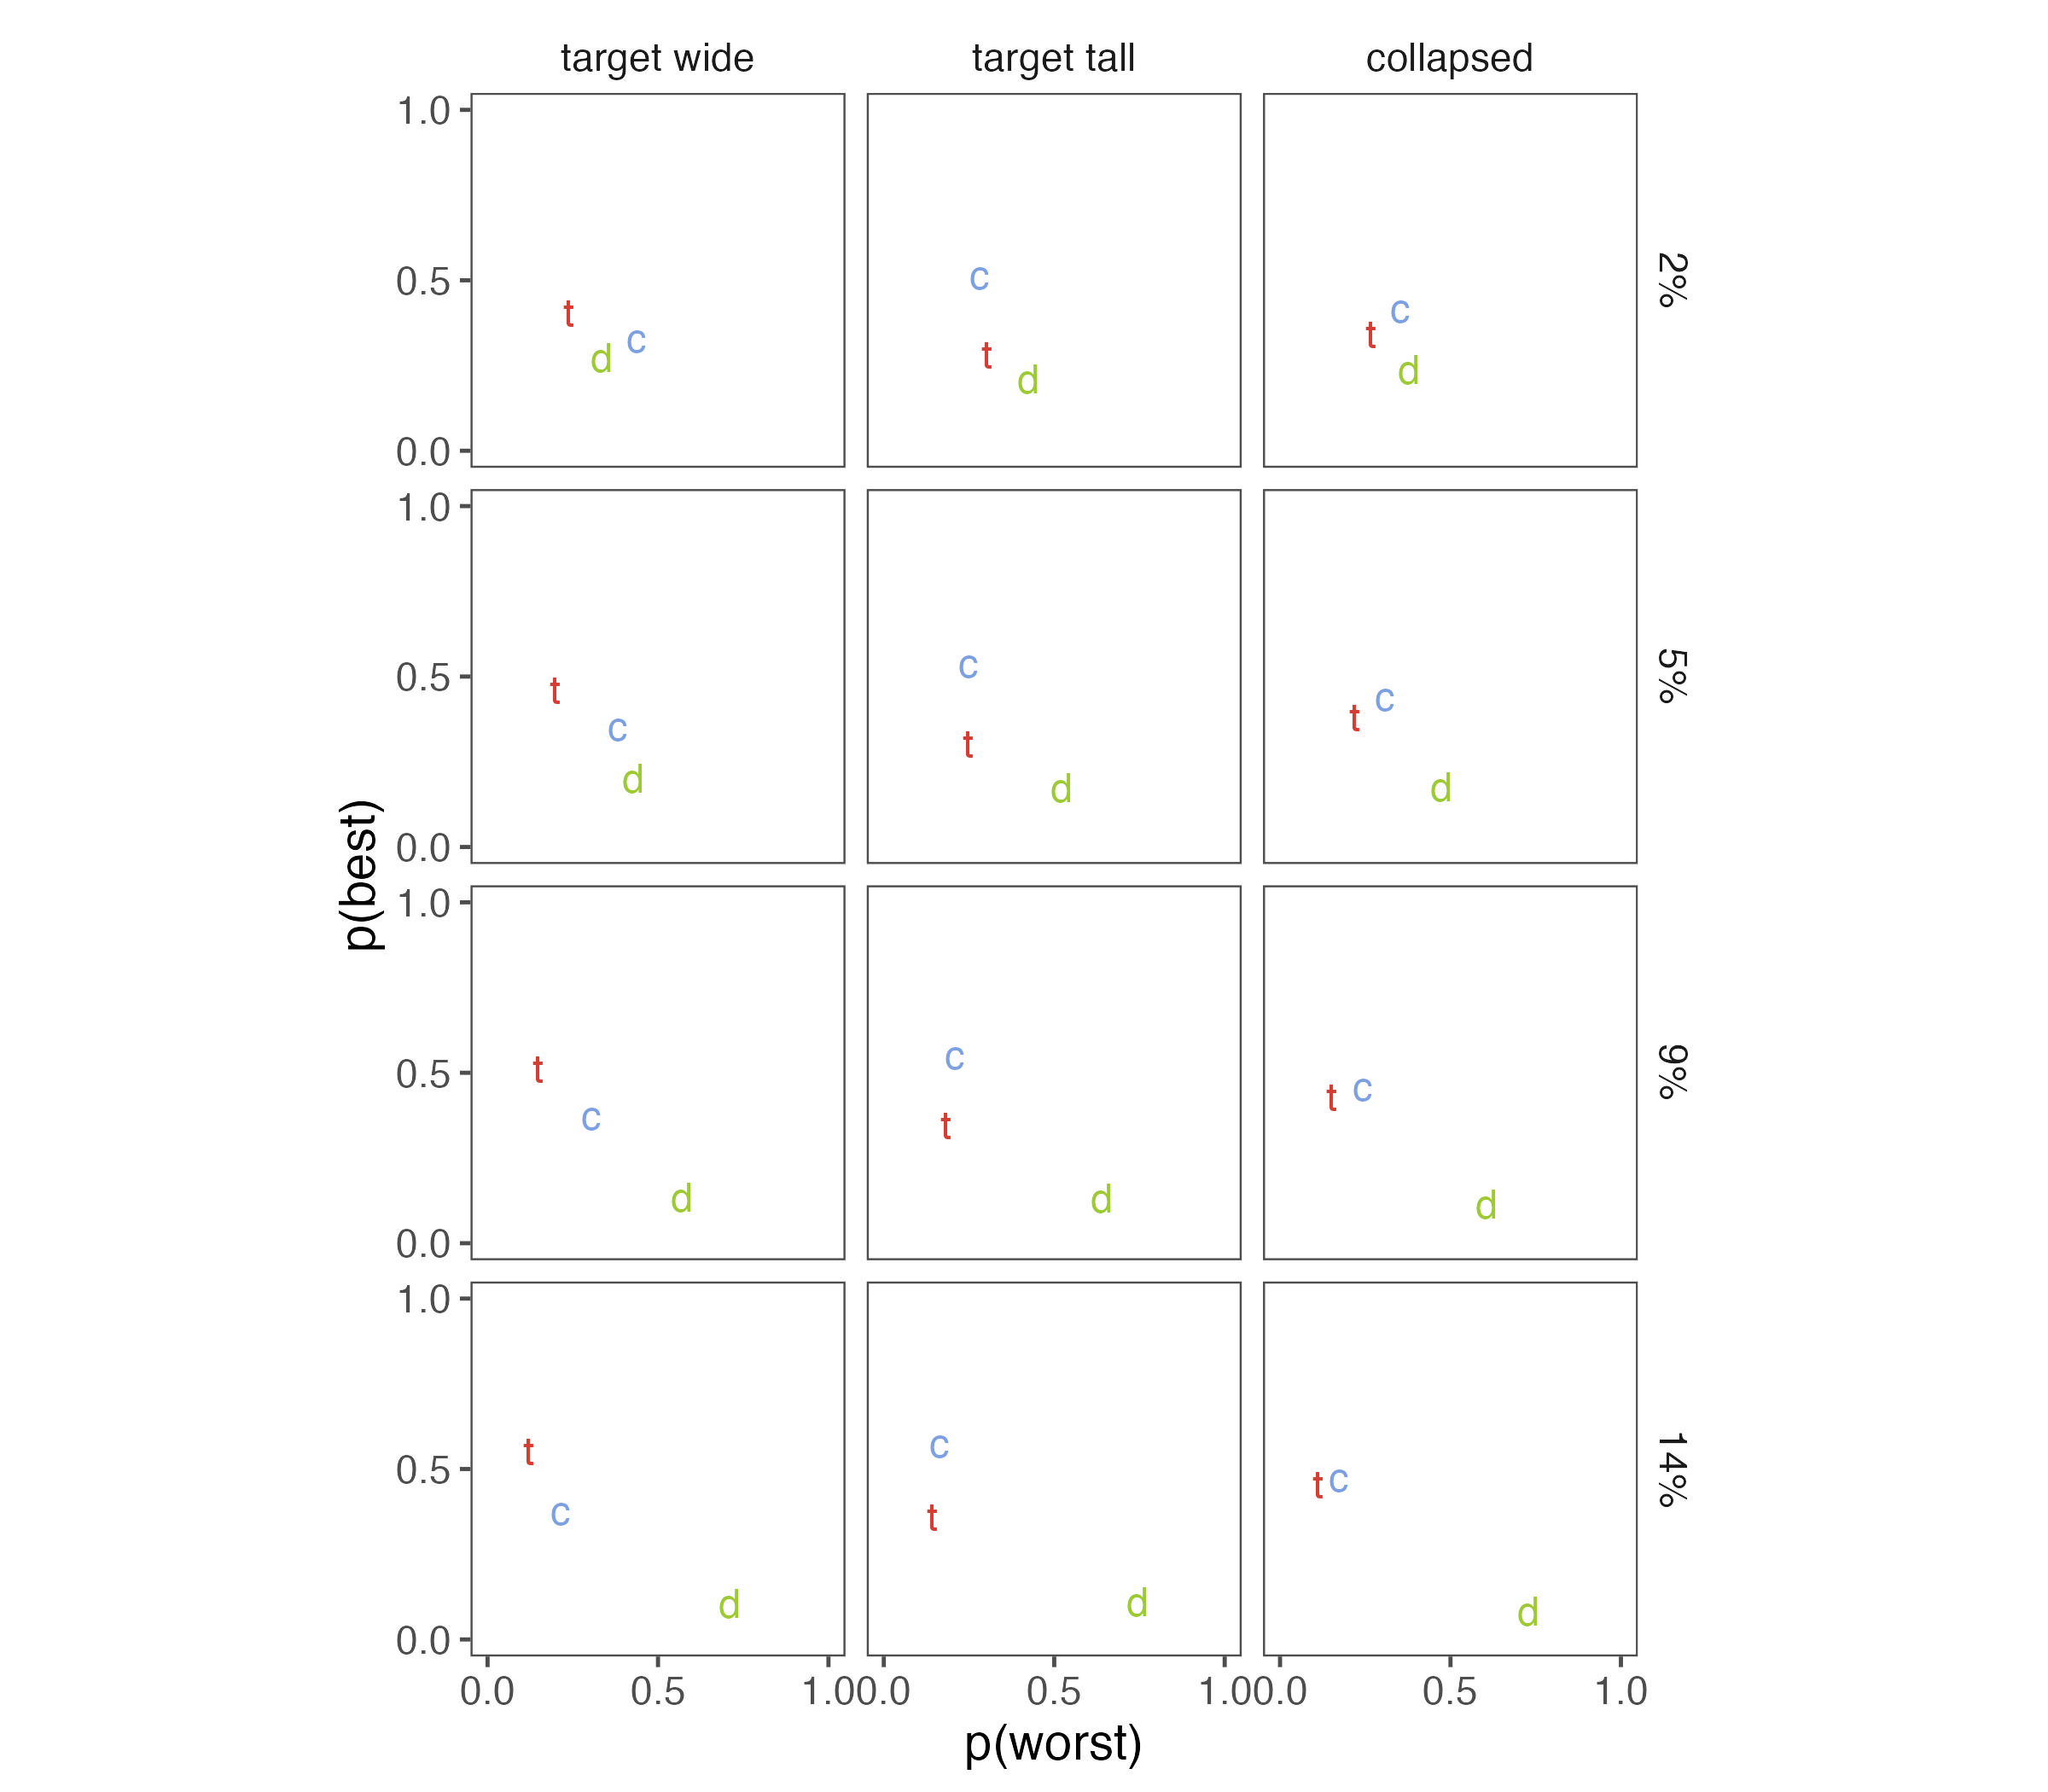
\includegraphics[width=170mm]{figures/crit_mean_props.jpeg}
   \caption{Experiment 3 mean best and worst-choice proportions, conditioned on TDD (rows) and choice set (columns). The left column shows data when the target was wide, the middle when the target was tall, while the right column collapses over orientation.}
   \label{fig:bw_mean_choice}
\end{figure}

Participants showed a consistent bias to choose $W$ (the wider rectangle) as largest, also found in Experiments 1, 2 and 5. Participants also (on average) regularly choose the decoy rectangle as smallest, except for the choice set $H,W,D_{W}$ and $TDD=2\%$, where they selected the $H$ rectangle as smallest, on average. This can be attributed to the difficulty of the $TDD=2\%$ condition and the overall wide rectangle bias. However, consistent with the predictions of the model, the target was still less likely to be chosen as worst than the competitor, $W(H|[H,W,D_{H}])<W(H|[H,W,D_{W}])$ and $W(W|[H,W,D_{W}])<W(W|[H,W,D_{H}])$, while the competitor option was also more likely to be chosen as best, $B(H|[H,W,D_{W}])>B(H|[H,W,D_{H}])$ and $B(W|[H,W,D_{H}])>B(W|{H,W,D_{W}})$. 

These results are more easily understood by plotting mean target, competitor, and decoy choice proportions across TDD levels, collapsed over choice set. See Figure~\ref{fig:bw_mean_choice} (right column) for these data. 

The best choice proportions replicated the results of \textcite{spektorWhenGoodLooks2018b} and the current Experiment 2, where the competitor was more likely to be chosen as best at low TDD levels, while competitor best-choice proportions also decreased with TDD. Decoy best-choice proportions also decreased systematically with TDD. Furthermore, the target was always less likely to be chosen as worst, compared to the competitor, at all TDD levels, $W(C)>W(T)$, as predicted by the Thurstonian choice model outlined in Chapter 2.

\subsubsection{Maxdiff Modeling}

Now consider the maxdiff model \parencite{marleyProbabilisticModelsBest2005}, which was outlined in the introduction to this chapter. This model predicts that the probability of choosing options $x$ as best and $y$ as worst, $x \neq y$, increases monotonically with the difference in their estimated utilities (see Equation~\ref{eqn:maxdiff_equation1}). This model is the most commonly used analysis technique for best-worst choice data \parencite{flynn2014best}. The maxdiff model was applied to the current experiment, where it is unable to predict the observed dissociations in best-worst choices, even with the best fitting parameter set.

Bayesian hierarchical model was used to fit the model. See the Appendix for the fitting procedure, including parameterization, priors, and parameter estimates. The model predictions for the mean best and worst choices are shown in Figure~\ref{fig:maxdiff_collapsed_preds}.

The model clearly mispredicts the data. The model predicts that the target and competitor are chosen at roughly equal amounts for both best and worst choice. Furthermore, note that the model predictions fall on a straight line rather than the curve shown by the data. This misprediction stems from the fact that the model choices are a function of the utility of each option, computed independently through a linear combination of experimental factors multiplied by model coefficients, including target/competitor/decoy status. The model could, if the data suggest it, predict that the target has greater utility than the competitor or vice versa. However, because best choice proportions are positively related to utility and worst choice proportions are negatively related to utility, the model cannot simultaneously predict $B(C)>B(T)$ and $W(T)<W(C)$. Instead, the mostly likely parameter set is that which predicts $B(C) \approx B(T)$ and $W(T) \approx W(C)$

Participant-level data and model predictions are shown in Figure~\ref{fig:maxdiff_sub_preds}. The model generally does a poor job at accounting for participant worst choice proportions.

\begin{figure}
   \centering
   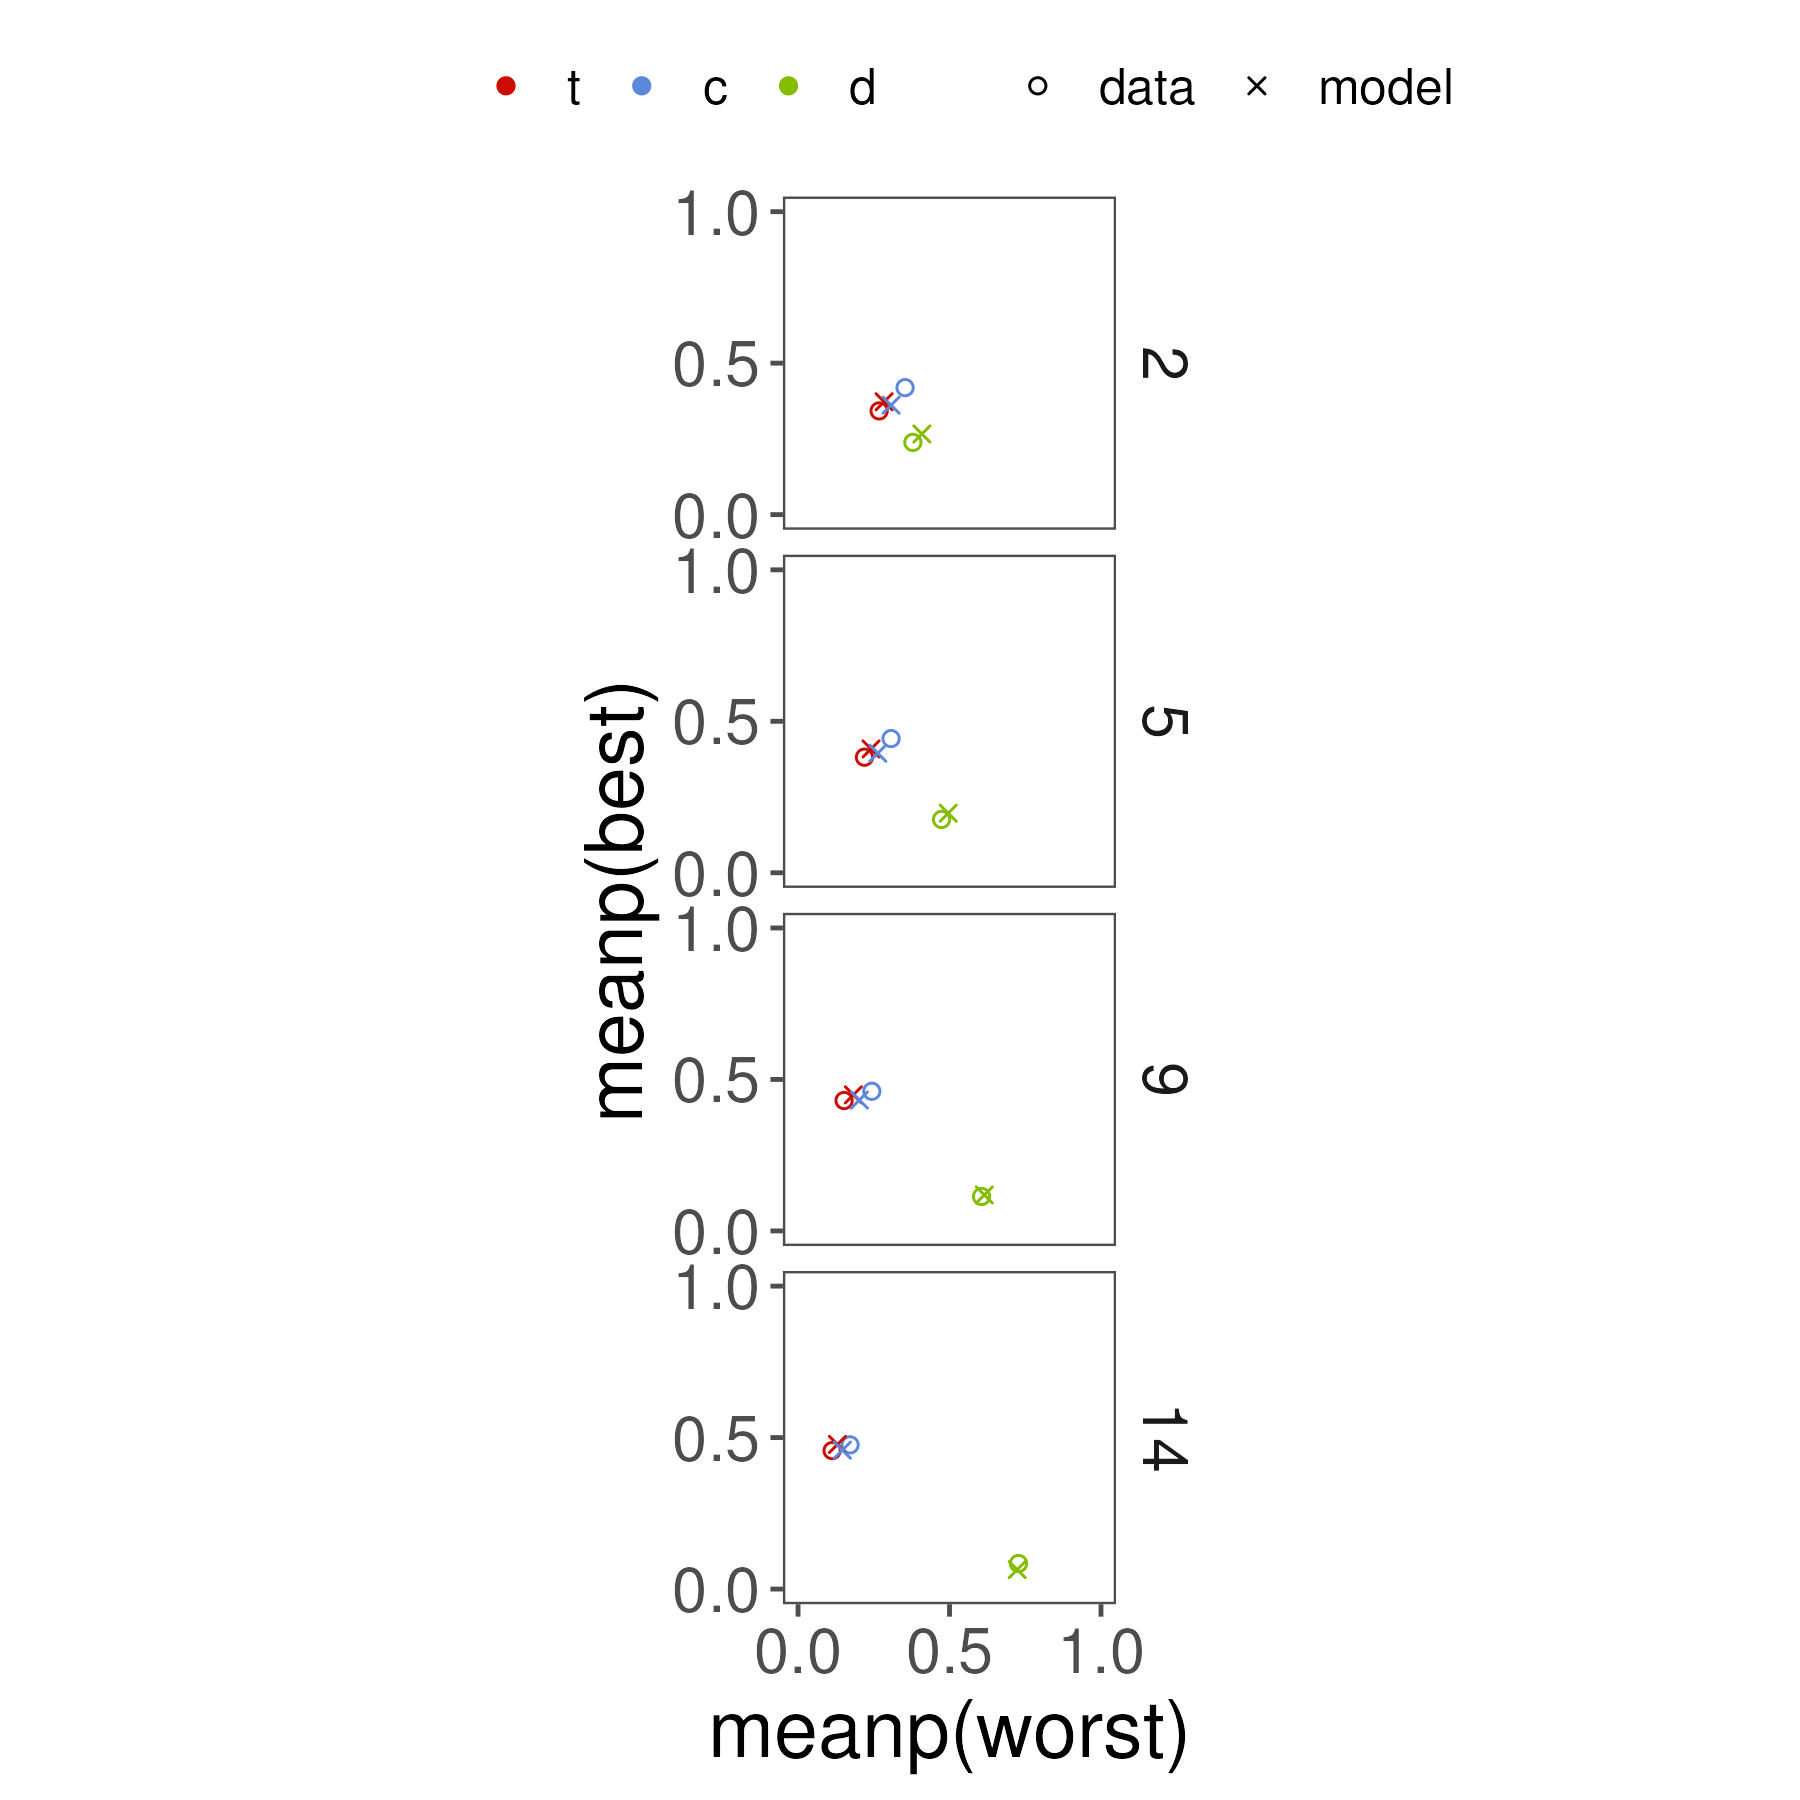
\includegraphics[width=\linewidth]{figures/maxdiff_1_means_model_v_data.jpeg}
   \caption{Experiment 3 maxdiff model predictions for the mean target, competitor, and decoy best-worst choice proportions. The model predictions fall on a single diagonal line, consistent with the monotonic best-worst choice predictions outlined earlier. Note that $95\%$ HDIs on the mean were too small to represent on the plot, but the data means are not included in any of these HDIs.}
   \label{fig:maxdiff_collapsed_preds}
\end{figure}

\begin{figure}
   \centering
   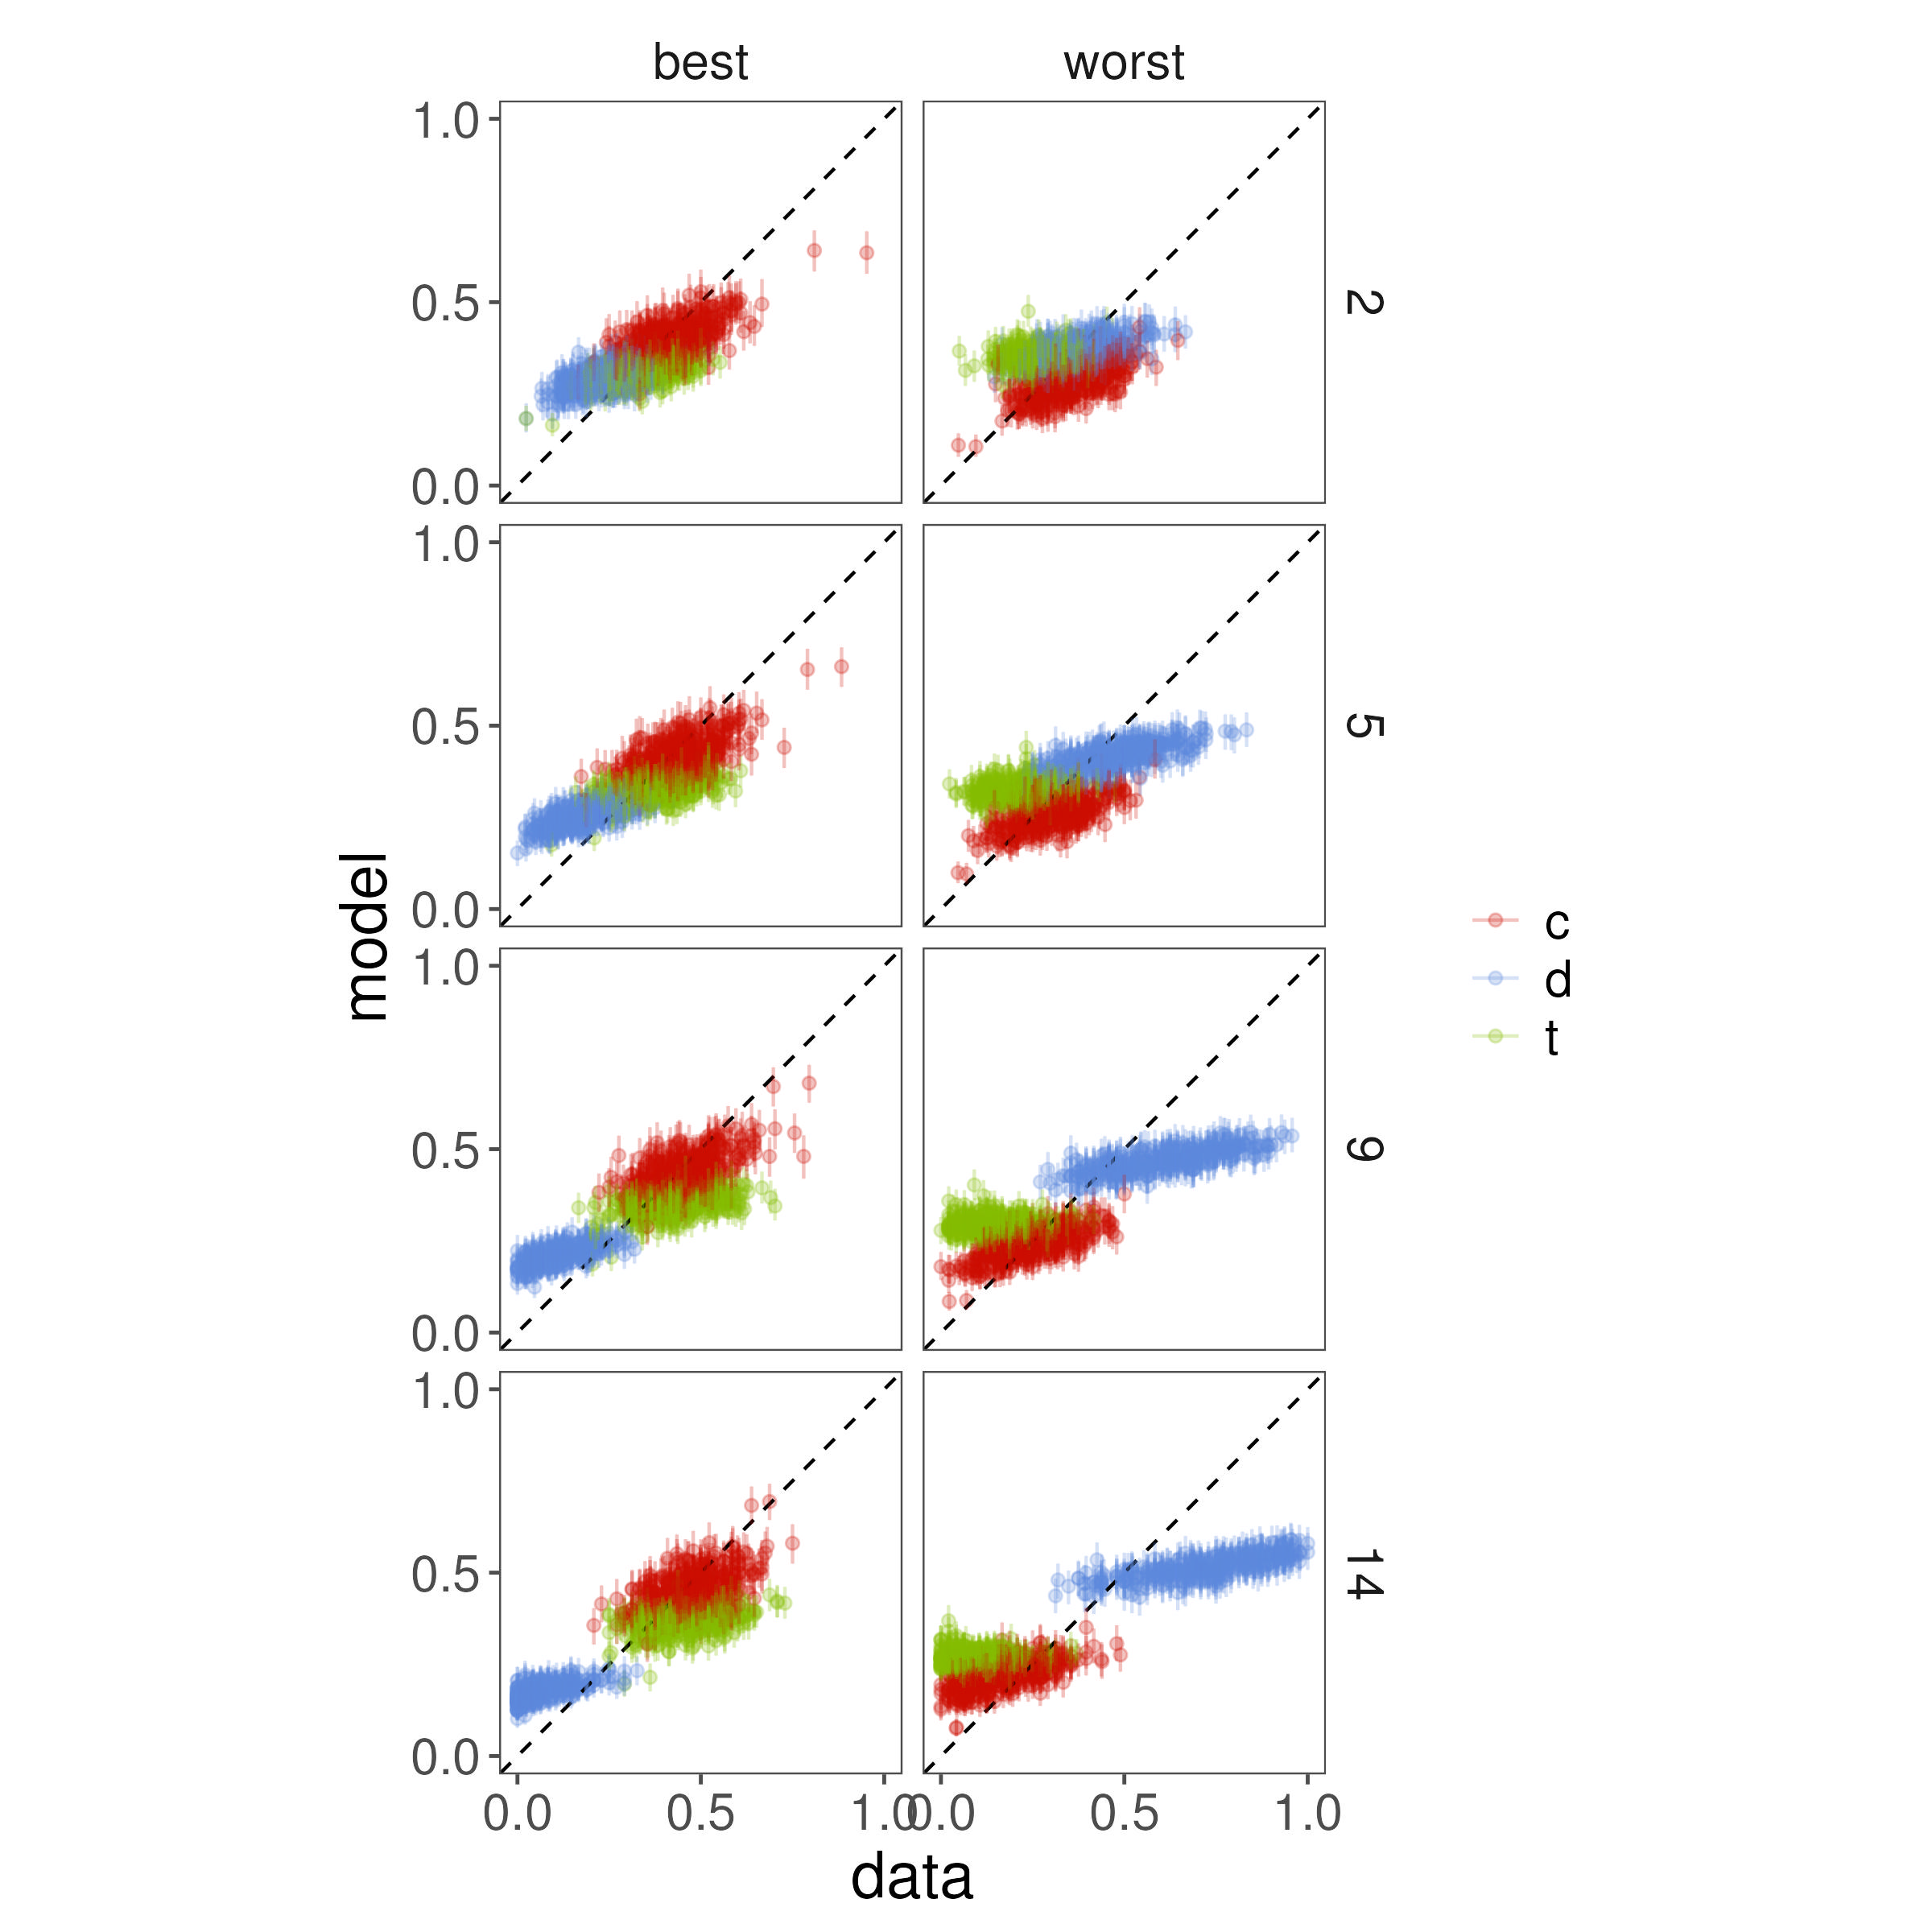
\includegraphics[width=\linewidth]{figures/maxdiff_1_subjectmeans_model_v_data.jpeg}
   \caption{Experiment 3 maxdiff model predictions for the mean target, competitor, and decoy best-worst participant-level choice proportions, conditioned on TDD (rows) and choice type, i.e. best v. worst (columns). Vertical error bars are $95\%$ HDIs.}
   \label{fig:maxdiff_sub_preds}
\end{figure}

\section{Discussion}
Experiment 3 demonstrated that correlated valuations can induce dissociations in best-worst choice. Specifically, given a target, competitor, and decoy option (borrowing the terminology of the attraction effect), the competitor is more likely than the target to be selected as best ($B(C)>B(T)$), but the competitor is also more likely than the target to be selected as worst ($W(C)>W(T)$). This prediction was made using the Thurstonian choice model of Chapter 2, conditioned on the parameters estimated from Experiment 3. Furthermore, the prediction was made with a different set of participants and a somewhat different experimental task. The maxdiff model, the most common model for best-worst choice analysis, cannot simultaneously predict $B(C)>B(T)$ and $W(C)>W(T)$.  

The maxdiff model assumes that, when selecting the best and worst option, the decision-maker picks the option with the highest and lowest utility, respectively. Most applications of the model assumes that these utilities are independently distributed \parencite{flynn2014best}, and that the decision-maker uses the same utility for both best and worst choices. The use of a single utility scale is to some extent a convenience assumption. \textcite{marleyProbabilisticModelsBest2005} explored several theoretical models, including the case where best and worst utilities exist on independent ratio scales, though such a model does not seem to have been adopted by substantive researchers. \textcite{marleyProbabilisticModelsSetdependent2008} introduced set-dependent best-worst choice models, which allow for context dependence based on choice set, albeit with best and worst choices still a function on a common underlying utility scale. 

\textcite{hawkins2019like} also argued that best and worst choices rely on a common utility representation, i.e., that the best option is chosen because it is highest in utility and the worst option is chosen because it is lowest in utility. They fit the maxdiff model to 5 best-worst datasets and showed, via Bayesian mixture modeling, that the overwhelming majority of participants were best fit by a model with a single utility representation. 

\textcite{gervzinivc2021estimating} argued (and provided evidence for) the claim that while best and worst choices rely on a common utility scale, people use two distinct decision rules for best choices and worst choices. They argued that the former is compensatory (i.e., allowing trade-offs between attributes), while the latter is non-compensatory (i.e., disallowing trade-offs to minimize future regret). 

The Thurstonian choice model, used for the current predictions, also employs a common utility scale for both best and worst choices. However, the model does not assume independently distributed utilities, as assumed by most applications of the maxdiff model. Thus, the claims of \textcite{hawkinsBestTimesWorst2014} and \textcite{hawkins2019like} are not necessarily falsified; rather, they are amended to account for correlations between option utilities. 
% I also replicated the main findings of \textcite{hawkinsBestTimesWorst2014}, that \textit{marginal} best and worst choice probabilities are monotonically related.

Due to the small effect size, this experiment required a large amount of data to estimate these dissociations. Most best-worst choice research is applied (for example in transportation and healthcare economics), where researchers do not typically have access a large amount of data at the individual participant level. Thus, researchers are unlikely to observe the dissociations in best-worst choice and will analyze the data using the maxdiff model. They may then arrive at incorrect conclusions regarding participants' preferences. 

% In a related paradigm, researchers have shown that allowing participants to reject all options from a set can affect choice. \textcite{tverskyChoiceConflictDynamics1992a} showed that people are more likely to reject all options if the options trade off on attributes compared to if one dominates the other. Other researchers have demonstrated that forced choice and free choice (when rejection is possible) can create markedly different choice patterns \parencite{dhar1997consumer,dhar1997context,dhar1996effect,dharEffectForcedChoice2003b,noguchiDescriptionexperienceGapChoice2016a,brazellNochoiceOptionDual2006b,parker2011rejectable,chernevChoiceOverloadConceptual2015}. 

The Thurstonian choice model was not fit to the Experiment 3 data. In Experiment 2, participants judged the size of the rectangles, and these judgments were used to estimate the model parameters. It also seems unreasonable to expect researchers to fit a multivariate Thurstonian model to most best-worst choice studies, given limitations in data and potential issues with parameter identifiability. 

The central purpose for conducting best-worst choice studies is to identify participants' preference distributions on a set of options. Best-worst choice is less cognitively demanding on participants than asking them to rank all options and far more efficient than pairwise forced choices on all combinations of options \parencite{louviere2008modeling}. In many cases, analyzing best-worst data with the maxdiff model may be the best approach, especially if researchers have no reason to believe that options are strongly correlated, or if all pairs of options have equally strong correlations. It is an open question, left for future research, whether correlations between options in applied choice research can create similar dissociations in best-worst choice. 

The maxdiff model's utility comes from its simplicity; it is essentially an extension of the MNL model to best-worst choice data. When choice sets are not designed to systematically various choice axioms (e.g., as in context effects), the MNL model is fairly effective in accounting for choice data; similarly, so is the maxdiff model effective in accounting for choice data where independence is not violated.

The current study only considered Case 3 best-worst choice \parencite{marleyModelsBestWorst2012}, where the attributes of options (in this case, height/width, TDD, diagonal) are systematically manipulated. This study did not consider Case 1 best-worst choice, where researchers are interested in preference for each option as a whole (e.g., a consumer's preference for cars over bicycles) or Case 2 best-worst choice, where researchers ask participants to select their preferred attribute from a set (e.g., a consumer's preference for short waiting times over physician experience in an urgent care clinic). Future research should consider ways to generalize the current paradigm and results to the other best-worst choice types.
